\chapter{Binocular Vision and Stereopsis}
\label{chap:BinocularVision}

\textit{Binocular vision} is a term used for the visual system of animals with two eyes \cite{how95}, and therefore, applies to the human visual system as well. 
Possessing binocular vision not only leads to a better perception of depth
of the surrounding environment, but also helps to better perform many visual tasks such as reading, object detection, interaction with surrounding objects such as grabbing and other manipulative 
tasks \cite{how95}. The most significant advantage of possessing binocular vision is its influence on how the 3D environment, that is, the 
depth of surrounding objects relative to each other, 
is perceived by the visual system. This visual perception of depth in binocular vision is referred to as {\it Stereoscopic Vision}.
In the visual system, depth perception is a phenomenon that normally occurs though different types of cues and information existing in the surrounding environment. 
These pieces of information, known as {\it depth cues} in stereo vision, can be either monocular or binocular depth cues \cite{how95}.
To name a few instances of monocular depth cues, we can refer to motion parallax, lighting and shading, and apparent size. 
However, as previously mentioned, binocular cues which can only be perceived
by stereo vision, play a major role in the perception of depth. One of the most important binocular cues is {\it binocular disparity}, or {\it binocular parallax}. 
It should be noted that the effect of binocular parallax and motion parallax on depth perception are very similar to each other. 
In motion parallax, which is a monocular depth cue, the scene is viewed at different times by the observer moving from one side to the other, 
whereas in binocular parallax, the scene is viewed from slightly different viewpoints at
the same time by the visual system, while the observer is standing at a fixed position \cite{how95}.

\begin{figure}[!h]
\centering
\subcaptionbox{Motion Parallax}
[.4\linewidth]{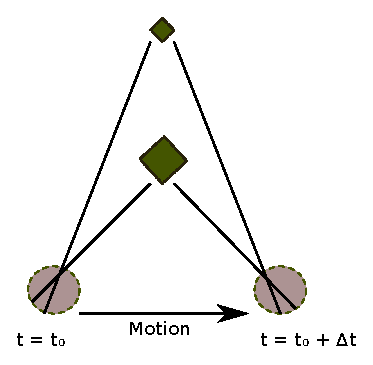
\includegraphics{Mparallax}}%
\subcaptionbox{Binocular Parallax}
[.4\linewidth]{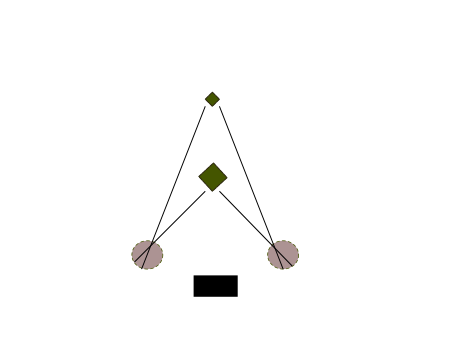
\includegraphics{Bparallax}}%
\caption{Motion parallax and binocular parallax difference}
\label{fig:parallax}
\end{figure}

%\begin{figure}[!h]
%\centering
%\begin{subfigure}[b]{7cm}            
%\frame{\includesvg[width=\textwidth]{Bparallax}}
%\caption{Interpolation for Data 1}
%\label{Fig:bp}
%\end{subfigure}
%
%\hspace{1cm}
%
%\begin{subfigure}[b]{7cm}
%\centering
%\frame{\includesvg[width=\textwidth]{Mparallax}}
%\caption{Interpolation for Data 2}
%\label{fig:mparallax}
%\end{subfigure}
%\caption{blah blah}\label{fig:bpmp}
%\end{figure}

Binocular disparity, which in fact arises from the spatial difference 
between the images of the same scene in the visual system, provides a relative perception of depth 
from the surrounding environment. This perception is known as {\it binocular stereopsis} \cite{how95}. 
Another important binocular depth cue is the eyes {\it vergence}, which is the simultaneous movement of the pupils in opposite directions in order to obtain a 
unified view of an object in the visual system. 
When focusing on an object, the optical axes of the eyes intersect on the object of interest resulting in an angle called vergence angle. 
The human visual system 
is capable of adjusting this angle based on the distance from the object \cite{how95}.
In stereo vision, the locus of the points that yield a unified view of an object in the visual system is 
known as the {\it horopter}, and any point located on the horopter is usually called a 
{\it fixation point} \cite{binr83,how95}.
An important property of an object on the horopter is that no spatial difference
exists between the images of the fixated object between the two eyes, that is, the binocular disparity is zero \cite{how95}. 
Exploiting this property, the disparity of any other object in the scene can be estimated relative to the fixated object by inspecting two important factors: 
whether the object of interest is closer or further than the fixated object and then how much closer or further it is relative to the fixated object.
As a result, the binocular disparity provides a relative perception of depth of the surrounding environment.
In the geometry of stereopsis, the relative disparity between two objects is usually presented as 
angular disparity in degrees, radians, minutes of arc (arcminute), 
or seconds of arc (arcsecond). The relation between these measurements is as follows:

\begin{align}
1 arcmin &= \frac{1}{60} degree = \frac{\pi}{10800} radians \label{eq:arcmin} \\
1 arcsecond &= \frac{1}{60} arcmin = \frac{1}{3600} degree = \frac{\pi}{648000} radians \label{eq:arcsec}
\end{align}

\section{Stereopsis Geometry and Angular Disparity}

In the following section, we will describe how the angular disparity can be calculated utilizing the geometry of stereopsis \cite{binr83}.

\begin{figure}[!h]
\centering
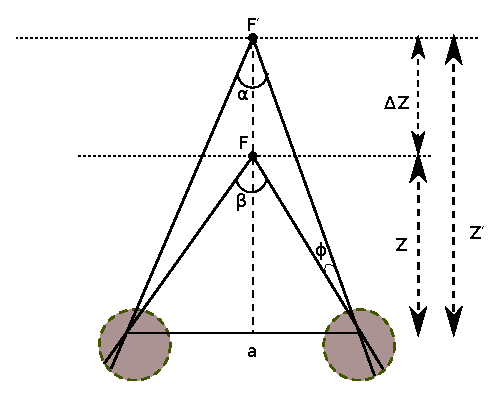
\includegraphics[width=0.5\textwidth]{binocular}
\caption{Binocular disparity}
\label{fig:stereopsis}
\end{figure} 

According to Figure \ref{fig:stereopsis}, we have:
\begin{align}
\label{eq:tang}
\tan \frac{\alpha}{2} &= \frac{a}{2Z^{'}}\\
\tan \frac{\beta}{2} &= \frac{a}{2Z}
\end{align}
It is known that for small angles, when the angle approaches zero, the tangent of an angle is approximately equal to the angle in radians. Therefore, we will
have the following relations:

\begin{align}
\theta &= 2\phi = \beta - \alpha\\
\frac{\alpha}{2} &\approx \frac{a}{2Z^{'}}\\
\frac{\beta}{2} &\approx \frac{a}{2Z}\\
Z^{'} &= Z + \Delta Z\\
\Rightarrow \theta &\approx \frac{a}{Z} - \frac{a}{Z^{'}}= \frac{a}{Z} - \frac{a}{Z+\Delta Z} \\
\Rightarrow \theta &\approx \frac{aZ+a\Delta Z-aZ}{Z(Z+\Delta Z)} = \frac{a \Delta Z}{Z(Z+ \Delta Z)}
\end{align}
When $\Delta Z$ is a small value compared to $Z$, the term $\Delta Z$ in the denominator can be neglected without 
significant loss of accuracy. This results in
the approximate formula as follows:

\begin{align}
\label{eq:stac}
\theta \approx \frac{a \Delta Z}{Z^{2}}
\end{align}

Here, $a$ is the distance between the center of the pupils of the two eyes, which is known as interpupillary distance.
It should be noted that $a$, $Z$ and $ \Delta Z$ must all have the same units in this formula. 
This equation estimates the angular disparity in radians; in order to convert $\theta$ to arcseconds, 
according to the conversion rules presented in Equation \ref{eq:arcsec}, it should be multiplied by:

\begin{align}
\frac {648000} {\pi} = 206,265 \frac{arcsec}{radians}
\end{align}

Studies show that the visual system capability to distinguish two objects at different depths relative to each other is limited to certain thresholds \cite{binr83,how95}.
This threshold, which is defined as the minimum detectable depth between two 
objects at difference distances, is known as {\it stereoacuity} which varies in different visual systems \cite{binr83,how95}. According to standard
stereo tests \cite{binr83}, the finest detectable disparity in the human visual system is approximately 10-15 arcseconds.
However, a more recent study on 60 subjects \cite{garn06} at different age groups, from 17 to 83 using standard stereotests, 
shows that the average stereoacuity for different age groups is as follows:

\begin{minipage}{\linewidth}
\begin{center}
\captionof{table}{Average stereoacuity for subjects of age 17 to 83}
\label{tab:stAcAge}
\begin{tabular}{ |c|c| }
\hline
\textbf{Age Range} & \textbf{Stereoacuity (arcsecs)} \\ \hline
17-29 & 32 \\  \hline
30-49 & 33.75 \\ \hline
50-69 & 38.75 \\ \hline
70-83 & 112.5 \\ \hline
\end{tabular}
\end{center}
\end{minipage} \newline

As can be seen, the stereoacuity for the the human visual system increases with age, that is, 
the amount of error in the depth results 
is less perceptible in the visual system of the elders than the youths.
Using these values in Equation \ref{eq:stac} along with the average interpupillary distance in the human visual system 
that is reported to be approximately $64$mm \cite{how95}, 
we can estimate the threshold for minimum detectable depth
between two objects based on their distance from the observer.

We have employed the concepts introduced in this chapter in the design of our evaluation model for an augmented reality system 
in outdoor environments.
In the next chapter, we will describe the design of our system and its components in more detail.
